\documentclass[9pt]{beamer}
\usepackage[utf8]{inputenc}
% \usepackage{algorithm,algorithmic}
% \usepackage{animate}

%Information to be included in the title page:
\title{Probabilitic Numerical Methods for Evaluating the Max Integral Operator}
\author{Nishad Gothoskar}
\institute{Learning and Intelligent Systems}
\date{July 27 2018}
 
\begin{document}
 
\frame{\titlepage}
 
\begin{frame}
\frametitle{Max Integral Operator}
In this work, we will explore techniques of estimating expressions of the following form:
\begin{equation*}
    \max_{a} \int f(a,s) \ \text{d}s
\end{equation*}
In high dimensions and continuous spaces, exact evaluation is many times intractable. As a result we have to take a probabilistic numerical approach to accurately and efficiently estimate its value.
\newline \newline
The Max Integral Operator is used in a variety of computational problems across many fields. In Reinforcement Learning it is used in MDPs for value update and POMDPs for belief updates. In inference problems we may use in computing the maximum a posteriori estimate.\newline \newline
Intuitively, maximizing over some parameters while integrating out others is a useful/important operation.
\end{frame}

\begin{frame}
\frametitle{Bayesian Quadrature}
Quadrature techniques, first presented as Bayes-Hermite Quadrature [1], are used to actively sample function evaluations in order to reduce uncertainty about an integral's value. This is usually done by maintaining a Gaussian Process over the integrand and then integrating the GP. 
\newline\newline
Most work in BQ has focused on integrals of the form:
\begin{equation*}
   \int f(x) p(x)  \ \text{d}x
\end{equation*}
In our framework, we will use this distribution over the integral's value as a convergence criterion, which can guide the optimization (maximization) procedure.
\end{frame}

\begin{frame}
\frametitle{Monte Carlo}
But why not use Monte Carlo to sample from $p$ and estimate the integral?
\newline\newline
Of course, with sufficiently many samples this will work. However, with a limited number of samples, by randomly sampling we might not be accurately represnting $f$. Quadrature selects this samples in order reduce our uncertainty about the integral's value.
\end{frame}

\begin{frame}
\frametitle{Basic Max Integral Optimization}
We will first demonstrate our method on a simple 2 dimensional function:
\begin{equation*}
\begin{split}
   f(s,a) &= \mathcal{N}(s | 3.0, 1.0) * \mathcal{N}(a | 0.0, 1.0) \\
   p(s) &= \mathcal{N}(s | 0.0, 10.0) \\
\end{split}
\end{equation*}
Now we will estimate:
\begin{equation*}
\begin{split}
   \max_{a} \int f(a,s) p(s) \ \text{d}s
\end{split}
\end{equation*}
\end{frame}

\begin{frame}
\frametitle{Basic Max Integral Optimization}
We take initial samples of $f(a,s)$ for each of actions. This gives us a rough estimate of the integral and serves as an initialization for the optimization.\newline \newline

Then we will proceed in a multi armed bandits fashion according to an acquisition function. Here, we use the UCB acquisition function. We find the $a^*$ that maximizes the acquisition function and then make queries to $f(\cdot , a^*)$. We combine this with the samples we already have (from previous iterations) in order to refind our estimate of the integral for that action.\newline \newline

We repeat the above procedure until some convergence criterion is satisfied. For this setting we have just discretized the action space. Later, we will present how to generalize this procedure to the continuous action setting.\newline \newline

probabilistic convergence criterion is reached (action $a^*$ is the argmax with probability $p$). Below is an animation showing execution of the optimization.
\end{frame}


\begin{frame}
\frametitle{Basic Max Integral Optimization}
Here are images of the progression of the algorithm.
\begin{figure}
   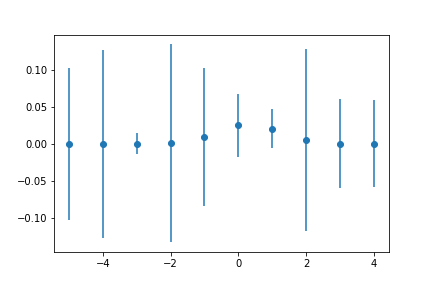
\includegraphics[width=0.3\textwidth]{im1}
   \hfill
   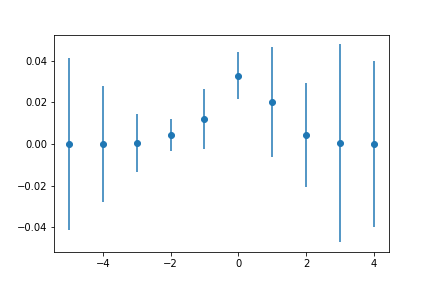
\includegraphics[width=0.3\textwidth]{im2}
   \hfill
   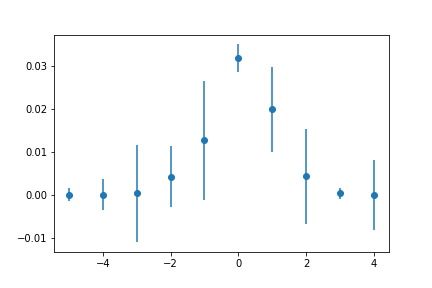
\includegraphics[width=0.3\textwidth]{im3}
\end{figure}
\end{frame}


\begin{frame}
\frametitle{Efficient Optimization}
In higher dimensions and larger spaces, quadrature (even in settings where there is a closed form solution) can be an expensive operation. By accounting for the distribution over value, we can focus on evaluating actions with potential of high value. As a result, the algorithm is sample efficient and feasible to implement in practice.\newline

This type of optimization procedure is necessary for evaluating the Max Integral operator. Without it, you will either sacrifice accuracy of the integral estimate (by discretization or Monte Carlo methods) or accuracy of the maximization procedure.\newline \newline
\end{frame}

\begin{frame}
\frametitle{Max Integral in RL}
In Reinforcement Learning, the Bellman Update (in continuous state space) is:

\[V^{\pi}(s) = \max_{a \in A} \int_{s' \in S} p(s'|s,a)\big(R(s'|s,a) + \gamma^{\Delta t}V^{\pi}(s')\big) \ \textup{d}s' \]

If we use a GP to model the Value Function, then we need to maximize over actions.\newline

From our experiments we see that it is infeasible to fully compute this integral for each action (each update is slow). We will use our optimization procedure in order to allow for more efficeint Bellman update. As a result, we are able to use GPs to model the value function and make more accurate value updates in each iterations.
\end{frame}



\begin{frame}
\frametitle{Bibliography}
[1] O’Hagan, A. (1991). Bayes–Hermite quadrature. Journal of Statistical Planning and Inference, 29(3), 245–260.\newline
[2]   M.  P.  Deisenroth,  J.  Peters,  and  C.  E.  Rasmussen,  “Approximate dynamic programming with Gaussian processes,” in Proc. of the IEEE American Control Conference (ACC), 2008, pp. 4480–4485.\newline
[3] Rasmussen, C.E., Ghahramani, Z.: Bayesian Monte Carlo. In Becker, S., Obermayer, K., eds.: Advances in Neural Information Processing Systems. Volume 15. MIT Press, Cambridge, MA (2003)
\end{frame}

 
\end{document}

